\documentclass[12pt,letterpaper]{scrartcl}
%\documentclass[12pt,letterpaper]{article}
\usepackage[margin=1in]{geometry}
\usepackage[superscript,biblabel]{cite}
\usepackage{url,graphicx,xcolor,enumitem}

%opening
\title{A Tutorial on PCB Design}
\subtitle{--- using KiCad}
\author{Xiaoguang ``Leo'' Liu, University of California Davis, lxgliu@ucdavis.edu}
\date{Aug.~9th, 2015}

\begin{document}

\maketitle

\tableofcontents

\newpage
\section{PCB Basics}

\subsection{Example 1: Arduino dice}

\subsection{Example 2: A 2.4\,GHz low noise amplifier (LNA)}

\section{KiCad}
In the early days, PCBs are designed and laid out literally by hand. See Fig.~\ref{fig:hand-pcb} for an example board from that era. As technologies developed, it become more common to do the job with the help of a computer. Today, there are numerous software tools for PCB design. On the high end, industry-grade packages, such as Cadence Allegro~\footnote{UC Davis students have access to the full suite of Allegro PCB design tools through a donation from Cadence.}, Mentor Graphics Xpedition, and Altium Designer, offer extensive features and capabilities with a high price tag and often a very steep learning curve. On the lower end, popular choices include CadSoft EAGLE, ExpressPCB, and DesignSpark, all of which offer a reasonable set of features at an affordable price. 

\begin{figure}[ht]
\centering
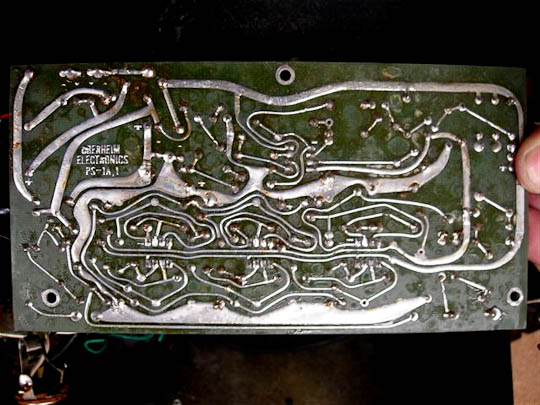
\includegraphics[width=3in]{hand-pcb.jpg}
\caption{A vintage PCB laid out by hand~\cite{hand-pcb}.}
\label{fig:hand-pcb}
\end{figure}

In recent years, KiCad has emerged as a popular open-source software package for designing and laying out PCBs~\cite{kicad}. KiCad is available on all three main personal computer operating systems, Windows, Linux, and Mac OS. 
Compared with the above mentioned software packages, KiCad is completely free of charge or any other limitation. Although KiCad is not as sophisticated as industry-level tools, it is capable of dealing with fairly complicated designs, and the active developer community is working hard to improve its capabilities. In fact, as of this writing, KiCad has not had an official stable release for the last two years. In this tutorial, we will using a recent build \#6055, dated Aug.~8th, 2015.


\section{Schematic Capture}

\subsection{Creating or Editing Schematic Symbols}
	
\section{PCB Layout}
\subsection{Associating schematic symbols with footprint}
\subsection{Creating or Editing Footprint}
\section{Generate Fabrication Files}
\section{Acknowledgment}

\newpage

\bibliography{kicad}
%\bibliographystyle{plain}

\end{document}
